\section{information retrieval}  

\subsection{introduction}


The meaning of the term information retrieval can be very broad. Just getting a credit card out of your wallet so that you can type in the card number is a form of information retrieval. However, as an academic field of study information retrieval might be defined thus: 

Information retrieval (IR) is finding material (usually documents) of an unstructured nature (usually text) that satisfies an information need from within large collections (usually stored on computers). As defined in this way, information retrieval used to be an activity that only a few people engaged in: reference librarians, paralegals, and similar professional searchers.

Now the world has changed, and hundreds of millions of people engage in information retrieval every day when they use a web search engine or search their email.1 Information retrieval is fast becoming the dominant form of information access, overtaking traditional database style searching (the sort that is going on when a clerk says to you:( “I’m sorry, I can only look up your order if you can give me your Order ID”).
 
IR can also cover other kinds of data and information problems beyond that specified in the core definition above. The term “unstructured data” refers to data which does not have clear, semantically overt, easy-for-a-computer structure. It is the opposite of structured data, the canonical example of which is a relational database, of the sort companies usually use to maintain product inventories and personnel records. In reality, almost no data are truly “unstructured”. This is definitely true of all text data if you count the latent linguistic structure of human languages. But even accepting that the intended notion of structure is overt structure, most text has structure, such as headings and paragraphs and footnotes, which is commonly represented in documents by explicit markup (such as the coding underlying web pages).

Information retrieval systems can also be distinguished by the scale at
which they operate, and it is useful to distinguish three prominent scales.
In web search, the system has to provide search over billions of documents
stored on millions of computers. Distinctive issues are needing to gather
documents for indexing, being able to build systems that work efficiently
at this enormous scale.




\subsection{Boolean retrieval model}

There are three simple retrieval methods. The first two methods produce ranked results, ordering the documents in the collection according to their expected relevance to the query. Our third retrieval method allows Boolean filters to be applied to the collection, identifying those documents that match a predicate.
 
Boolean filters applied by Web search engines, explicit support for Boolean queries is important in specific application areas such as digital libraries and the legal domain. In contrast to ranked retrieval, Boolean retrieval returns sets of documents rather than ranked lists.

Under the Boolean retrieval model, a term t is considered to specify the set of documents containing it,where The result of a Boolean query is a set of documents matching the predicate,and The standard Boolean operators (AND, OR, and NOT)are used to construct Boolean queries.

You may wonder why we represent these queries as vectors rather than sets. Representation as a vector is useful when terms are repeated in a query and when the ordering of terms is significant. In ranking formulae, we use the notation qt to indicate the number of times term t appears in the query.

There is a key difference in the conventional interpretations of term vectors for ranked retrieval and predicates for Boolean retrieval. Boolean predicates are usually interpreted as strict filters ,if a document does not match the predicate, it is not returned in the result set. Term vectors, on the other hand, are often interpreted as summarizing an information need. Not all the terms in the vector need to appear in a document for it to be returned. 

\subsection{AD Hoc retrieval}

We assume an average of 6 bytes perword including spaces and punctuation,
then this is a document collection about 6 GB in size. Typically, there might
be about M = 500,000 distinct terms in these documents. 

There is nothing special about the numbers we have chosen, and they might vary by an order of magnitude or more, but they give us some idea of the dimensions of the
kinds of problems we need to handle. 

Because the number of possible queries is huge ; Our goal is to develop a system to address the ad hoc retrieval task. This is the most standard IR task. In it, a system aims to provide documents from within the collection that are relevant to an arbitrary user information need, communicated to the system by means of a one-off, user-initiated query.


\subsection{inverted index}

An inverted index is index always maps back from terms to the parts of a document where they occur. Nevertheless, inverted index, or sometimes inverted file, has become the standard termin information retrieval.
 
\subsubsection{A first take at building an inverted index}

\begin{figure}[H]%
    \center%
    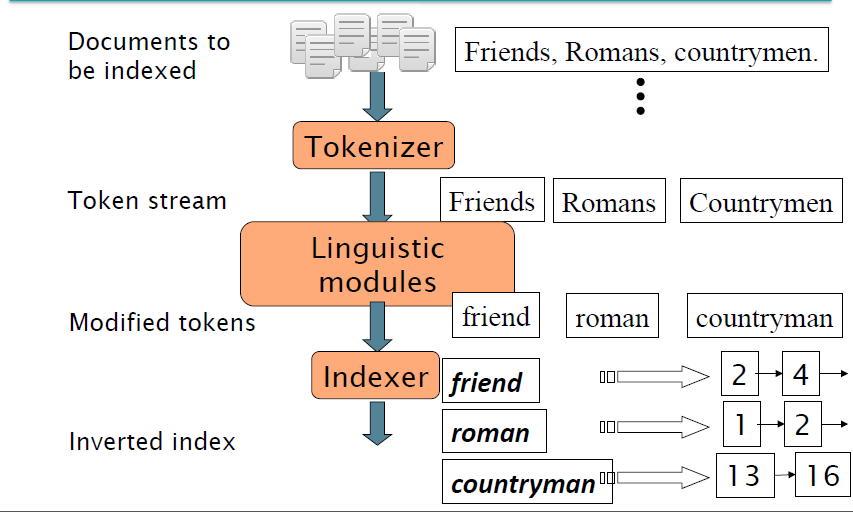
\includegraphics[width=0.6\textwidth]{images/shimaa/building an inverted index.png}
     % you need to add the caption for the list of figures
    \caption[This is building an inverted index]{building an inverted index}\label{fig:building an inverted index}%
\end{figure}
 
To gain the speed benefits of indexing at retrieval time, we have to build the
index in advance. The major steps in this are:

1.Collect the documents to be indexed.

2.Tokenize the text, turning each document into a list of tokens.

3.Do linguistic preprocessing , producing a list of normalized tokens, which
  are the indexing terms.
  
4.Index the documents that each term occurs in by creating an inverted index,
  consisting of a dictionary and postings.

\begin{itemize}
     \item \textbf{Tokenization}\\
     Given a character sequence and a defined document unit, tokenization is the
     task of chopping it up into pieces, called tokens, perhaps at the same time
     throwing away certain characters, such as punctuation.
     
     
     \item \textbf{Dropping common terms: stop words}\\
     Sometimes, some extremely common words which would appear to be of
     little value in helping select documents matching a user need are excluded
     from the vocabulary entirely.
     The general strategy for determining a stop list is to sort the terms by collection frequency (the total number of times each term appears in the document collection),and then to take the most frequent terms, often hand-filtered for their semantic content relative to the domain of the documents being indexed.
     
     
     \item  \textbf{Normalization}\\ 
     Having broken up our documents (and also our query) into tokens, the easy
     case is if tokens in the query just match tokens in the token list of the document.
     
     There are many cases when two character sequences are not quite the same but you would like a match to occur. For instance, if you search for USA, you might hope to also match documents containing U.S.A .
     
     Token normalization is the process of canonicalizing tokens so that matches occur despite superficial differences in the character sequences of the to kens.
    
    \item  \textbf{stemming}\\
    For grammatical reasons, documents are going to use different forms of a word,such as organize,organizes,and organizing. Additionally,there are families of derivationally related words with similar meanings,such as democracy, democratic, and democratization. In many situations, it seems as if it would be useful for a search for one of these words to return documents that contain another word in the set.
    
    The goal of both stemming is to reduce inflectional forms and sometimes derivationally related forms of a word to a common base form.
    For instance:
    
    am, are,is \Rightarrow  be \\
    
    car, cars, car’s, cars’ \Rightarrow  car \\
      
    
    The result of this mapping of text will be something like:\\
      
    
    the boy’s cars are different colors  \Rightarrow   the  boy  car  be  differ   color
      
      
\end{itemize} 

\subsection{ranked retrieval}

We have dealt with indexes that support Boolean queries: a document
either matches or does not match a query. In the case of large document
collections, the resulting number of matching documents can far exceed the
number a human user could possibly sift through. Accordingly, it is essential
for a search engine to rank-order the documents matching a query. 
To do this, the search engine computes, for each matching document, a score with
respect to the query at hand. 
we initiate the study of assigning a score to a ( query, document ) pair.

\subsubsection{term frequency}

We assign to each term in a document a weight for that term, that depends on the number of occurrences of the term in the document.

We would like to compute a score between a query term t and a document d, based on the weight of t in d. The simplest approach is to assign the weight to be equal to the number of occurrences of term t in document d.
This weighting scheme is referred to as term frequency with the subscripts denoting the term and the document in order.

For a document d, the set of weights determined by the tf weights above
(or indeed any weighting function that maps the number of occurrences of t
in d to a positive real value) may be viewed as a quantitative digest of that
document.


\begin{itemize}
     \item \textbf{The log frequency weight of term t in d is}\\
\begin{equation}
        \large 
           W_{t,d} =\left\{ \begin{array}{c1} 1+\log_{10}(tf_{t,d}) & \text{if  } 
           tf_{t,d} > 0 \\ 0 & \text{otherwise.} \end{array}\right.\end{equation}
\end{itemize}


\begin{itemize}
     \item \textbf{Bag of words}\\
     In this view of a document, known in the literature as the bag
     of words model, the exact ordering of the terms in a document is ignored but
     the number of occurrences of each term is material (in contrast to Boolean
     retrieval). 
     We only retain information on the number of occurrences of each term. 
    
     The document “Mary is quicker than John” is, in this view, identical to the document “John is quicker than Mary”. it seem intuitive that two documents with similar bag of words representations are
     similar in content.
\end{itemize} 

\subsubsection{inverse document frequency}

term frequency as above suffers from a critical problem: all terms are
considered equally important when it comes to assessing relevancy on a
query. 

In fact certain terms have little or no discriminating power in determining
relevance. For instance, a collection of documents on the auto
industry is likely to have the term auto in almost every document.
we introduce a mechanism for attenuating the effect of terms that occur
too often in the collection to be meaningful for relevance determination.


How is the document frequency df of a term used to scale its weight? 
Denoting as usual the total number of documents in a collection by N,we define the inverse document frequency \( idf \) of a term t as follows:

\begin{equation}
        \large 
            idf_{t} = \log (N | df_{t})\end{equation}

\subsubsection{tf-idf weighting}

We now combine the definitions of term frequency and inverse document
frequency, to produce a composite weight for each term in each document.

The tf-idf weighting scheme assigns to term t a weight in document d given
by
\begin{equation}
    \large
     tf-idf_{t,d} = tf_{t,d } * idf_{t} \end{equation}  
     
In other words, tf-idf t,d assigns to term t a weight in document d that is

1. highest when t occurs many times within a small number of documents
(thus lending high discriminating power to those documents).

2. lower when the term occurs fewer times in a document, or occurs in many
documents (thus offering a less pronounced relevance signal).

3. lowest when the term occurs in virtually all documents.     

\begin{itemize}
     \item \textbf{Document Vector}\\
    At this point, we may view each document as a vector with one component
    corresponding to each term in the dictionary, together with a weight for each
    component that is given by (4.3). For dictionary terms that do not occur in
    a document, this weight is zero. This vector form will prove to be crucial to
    scoring and ranking .

    As a first step, we introduce the overlap score measure: the score of a document d is the sum, over all query terms, of the number of times each of the query terms occurs in d. We can refine this idea so that we add up not the number of occurrences of each query term t in d, but instead the tf-idf weight of each term in d.
   
   \begin{equation}
        \large
         \text{score}(q,d) =\sum tf-idf_{t,d}. \end{equation}
\end{itemize}


\subsection{The vector space model for scoring}

We developed the notion of a document vector that captures the relative importance of the terms in a document. 
The representation of a set of documents as vectors in a common vector space is known as the vector space model and is fundamental to a host of information retrieval operations ranging from scoring documents on a query, document classification and document clustering.

\begin{itemize}
     \item \textbf{Dot products}\\
     We denote by V(d) the vector derived from document d, with one component in the vector for each dictionary term. Unless otherwise specified,the reader may assume that the components are computed using the tf-idf weighting scheme, although the particular weighting scheme is immaterial to the discussion that follows: 
     The set of documents in a collection then may be viewed as a set of vectors in a vector space, in which there is one axis for each term.              This representation loses the relative ordering of the terms in each document.
      
     
\end{itemize}

\begin{itemize}
     \item \textbf{Euclidean distance}\\
     distance between two points (distance between the end points of the two vectors). 
     Euclidean distance is a bad idea because Euclidean distance is large for vectors of different lengths.
     
     
\begin{figure}[H]%
    \center%
    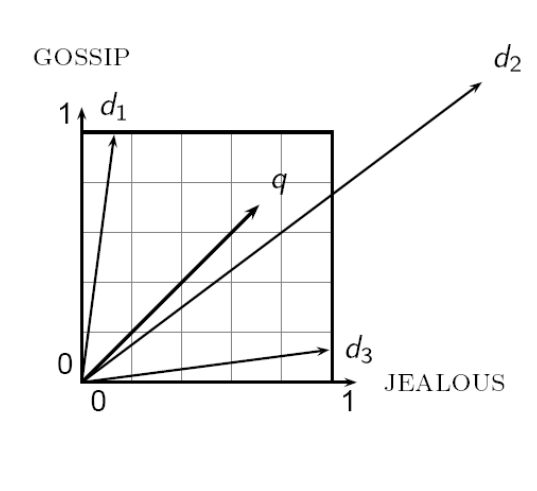
\includegraphics[width=0.6\textwidth]{images/shimaa/Euclidean distance.png}
     % you need to add the caption for the list of figures
    \caption[This is Euclidean distance]{Euclidean distance}\label{fig:Euclidean distance}%
   \end{figure}

   The Euclidean distance between\displaystyle  $$\vec{q} \textrm{ and }\vec{d2 } \textrm{  is large even though the distribution of terms in the query}\\ \displaystyle \vec{q}\textrm{  and the distribution of terms in the document} \vec{d2} \textrm {  are very similar}$$.  
  
\end{itemize}   

\subsection{cosine similarity}

How do we quantify the similarity between two documents in this vector
space? A first attempt might consider the magnitude of the vector difference
between two document vectors.
This measure suffers from a drawback: two documents with very similar content can have a significant vector difference simply because one is much longer than the other. Thus the relative distributions of terms may be identical in the two documents, but the absolute term frequencies of one may be far larger.

To compensate for the effect of document length, the standard way of
quantifying the similarity between two documents d1 and d2 is to compute
the cosine similarity of their vector representations \displaystyle $$\vec{V}(d_1) \textrm{and} \vec{V}(d_2) $$.

\begin{equation}
    \large
         \text{sim}(d_1 ,d_2) \\
         =\frac{\vec{V}( d_1 ) . \vec{V}( d_2 ) } {|\vec{V}( d_1 )| |\vec{V}( d_2 )|}
\end{equation}


The effect of the denominator of Equation (4.5) is thus to length-normalize
the vectors \displaystyle $$\vec{V}(d_1) \textrm{and}\vec{V}(d_2)
\textrm{ to unit vectors } \vec{V}(d_1) = \vec{V}(d_1) /|\vec{V}(d_2)|  \textrm{and} \vec{V}(d_2) = \vec{V}(d_1) .|\vec{V}(d_2)|$$.

